% questions.tex —— 2008 年·普通高等学校招生考试·福建卷·理科 · 题目内容片段（无答案）
% 由 tools/generate_projects.py 依来源总账自 2008/2008_数学真题_福建理_试题.md 生成，勿手改（改源 MD 后重跑）


\gkpart{一、选择题}

\begin{question}
\gkti{1}若复数 $(a^2-3a+2)+(a-1)\mathrm i$ 是纯虚数，则实数 $a$ 的值为（　）

（A）$1$

（B）$2$

（C）$1$ 或 $2$

（D）$-1$

\end{question}
\begin{question}
\gkti{2}设集合 $A=\left\{x\mid \dfrac{x}{x-1}<0\right\}$，$B=\{x\mid 0<x<3\}$，那么“$m\in A$”是“$m\in B$”的（　）

（A）充分而不必要条件

（B）必要而不充分条件

（C）充要条件

（D）既不充分也不必要条件

\end{question}
\begin{question}
\gkti{3}设 $\{a_n\}$ 是公比为正数的等比数列，若 $a_1=7$，$a_5=16$，则数列 $\{a_n\}$ 前 $7$ 项的和为（　）

（A）$63$

（B）$64$

（C）$127$

（D）$128$

\end{question}
\begin{question}
\gkti{4}函数 $f(x)=x^3+\sin x+1$（$x\in\mathbf R$），若 $f(a)=2$，则 $f(-a)$ 的值为（　）

（A）$3$

（B）$0$

（C）$-1$

（D）$-2$

\end{question}
\begin{question}
\gkti{5}某一批花生种子，如果每 $1$ 粒发芽的概率为 $\dfrac45$，那么播下 $4$ 粒种子恰有 $2$ 粒发芽的概率是（　）

（A）$\dfrac{16}{625}$

（B）$\dfrac{96}{625}$

（C）$\dfrac{192}{625}$

（D）$\dfrac{256}{625}$

\Needspace{0.4\textheight}
\end{question}
\begin{question}
\gkti{6}如图，在长方体 $ABCD-A_1B_1C_1D_1$ 中，$AB=BC=2$，$AA_1=1$，则 $BC_1$ 与平面 $BB_1D_1D$ 所成角的正弦值为（　）

（A）$\dfrac{\sqrt6}{3}$

（B）$\dfrac{2\sqrt6}{5}$

（C）$\dfrac{\sqrt{15}}{5}$

（D）$\dfrac{\sqrt{10}}{5}$
\nopagebreak[4]
\begin{center}% 2008 年福建卷理科第 6 题：长方体 ABCD-A1B1C1D1，AB=BC=2，AA1=1，
%   求 BC1 与平面 BB1D1D 所成角的正弦值。
% 来源 PDF：gaokaomath-src/普通高考/2008/2008福建理.pdf
% SHA-256：516e8ac8e113868afa9bc4af4724c3b43f22a1f7fecc830a7f3400b8d973d452
% 原页：2008福建理.pdf 第 1 页（A3 三栏）第 1 栏，书页码 441。
% 重绘依据：按原页斜投影：A 前左下、B 前右下、C 右侧、D 被遮挡；A1、B1、C1、D1 为对应顶点；
%   A—D、D—C、D—D1、B—D 虚线，其余棱与对角线 BC1 实线。
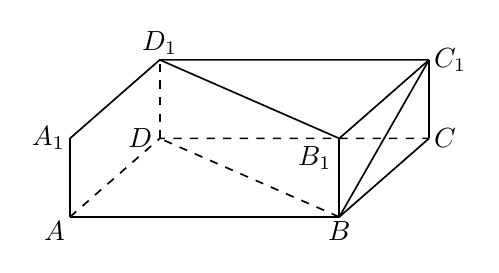
\begin{tikzpicture}[scale=0.95, semithick, every node/.style={inner sep=1.5pt}]
  \coordinate (A) at (0.00,0.00);
  \coordinate (B) at (3.60,0.00);
  \coordinate (C) at (4.80,1.05);
  \coordinate (D) at (1.20,1.05);
  \coordinate (A1) at (0.00,1.05);
  \coordinate (B1) at (3.60,1.05);
  \coordinate (C1) at (4.80,2.10);
  \coordinate (D1) at (1.20,2.10);

  \draw (A) -- (B) -- (C);
  \draw (A) -- (A1);
  \draw (B) -- (B1);
  \draw (C) -- (C1);
  \draw (A1) -- (D1) -- (C1);
  \draw (D1) -- (B1);
  \draw (B1) -- (C1);
  \draw (B) -- (C1);

  \draw[dashed] (A) -- (D) -- (C);
  \draw[dashed] (D) -- (D1);
  \draw[dashed] (B) -- (D);

  \node[below left] at (A) {$A$};
  \node[below] at (B) {$B$};
  \node[right] at (C) {$C$};
  \node[left=1pt] at (D) {$D$};
  \node[left] at (A1) {$A_1$};
  \node[below left=1pt] at (B1) {$B_1$};
  \node[right] at (C1) {$C_1$};
  \node[above] at (D1) {$D_1$};
\end{tikzpicture}
\end{center}
\nopagebreak[4]
\end{question}
\begin{question}
\gkti{7}某班级要从 $4$ 名男生、$2$ 名女生中选派 $4$ 人参加某次社区服务，如果要求至少有 $1$ 名女生，那么不同的选派方案种数为（　）

（A）$14$

（B）$24$

（C）$28$

（D）$48$

\end{question}
\begin{question}
\gkti{8}若实数 $x$、$y$ 满足 $\begin{cases}x-y+1\leqslant0,\\ x>0,\end{cases}$ 则 $\dfrac yx$ 的取值范围是（　）

（A）$(0,1)$

（B）$(0,1]$

（C）$(1,+\infty)$

（D）$[1,+\infty)$

\end{question}
\begin{question}
\gkti{9}函数 $f(x)=\cos x$（$x\in\mathbf R$）的图象按向量 $(m,0)$ 平移后，得到函数 $y=-f'(x)$ 的图象，则 $m$ 的值可以为（　）

（A）$\dfrac{\pi}{2}$

（B）$\pi$

（C）$-\pi$

（D）$-\dfrac{\pi}{2}$

\end{question}
\begin{question}
\gkti{10}在 $\triangle ABC$ 中，角 $A$、$B$、$C$ 的对边分别为 $a$、$b$、$c$。若 $(a^2+c^2-b^2)\tan B=\sqrt3ac$，则角 $B$ 的值为（　）

（A）$\dfrac{\pi}{6}$

（B）$\dfrac{\pi}{3}$

（C）$\dfrac{\pi}{6}$ 或 $\dfrac{5\pi}{6}$

（D）$\dfrac{\pi}{3}$ 或 $\dfrac{2\pi}{3}$

\end{question}
\begin{question}
\gkti{11}双曲线 $\dfrac{x^2}{a^2}-\dfrac{y^2}{b^2}=1$（$a>0$，$b>0$）的两个焦点为 $F_1$、$F_2$，若 $P$ 为其上一点，且 $|PF_1|=2|PF_2|$，则双曲线离心率的取值范围为（　）

（A）$(1,3)$

（B）$(1,3]$

（C）$(3,+\infty)$

（D）$[3,+\infty)$

\Needspace{0.4\textheight}
\end{question}
\begin{question}
\gkti{12}已知函数 $y=f(x)$，$y=g(x)$ 的导函数的图象如下图，那么 $y=f(x)$，$y=g(x)$ 的图象可能是（　）
\nopagebreak[4]
\begin{center}% 2008 年福建卷理科第 12 题：已知 y=f(x)、y=g(x) 的导函数图象（f' 递减、g' 递增，
%   在 x=x0 处相交），选 f、g 的图象可能的一组。
% 来源 PDF：gaokaomath-src/普通高考/2008/2008福建理.pdf
% SHA-256：516e8ac8e113868afa9bc4af4724c3b43f22a1f7fecc830a7f3400b8d973d452
% 原页：2008福建理.pdf 第 1 页（A3 三栏）第 2 栏，书页码 441。
% 绘制依据：f' 递减、g' 递增且在 x0 相交，故 f-g 在 x0 取极大；四组候图中只有 (C)
%   满足两曲线在 x0 处相切且 f 在 g 下方，与原页排成 2×2。
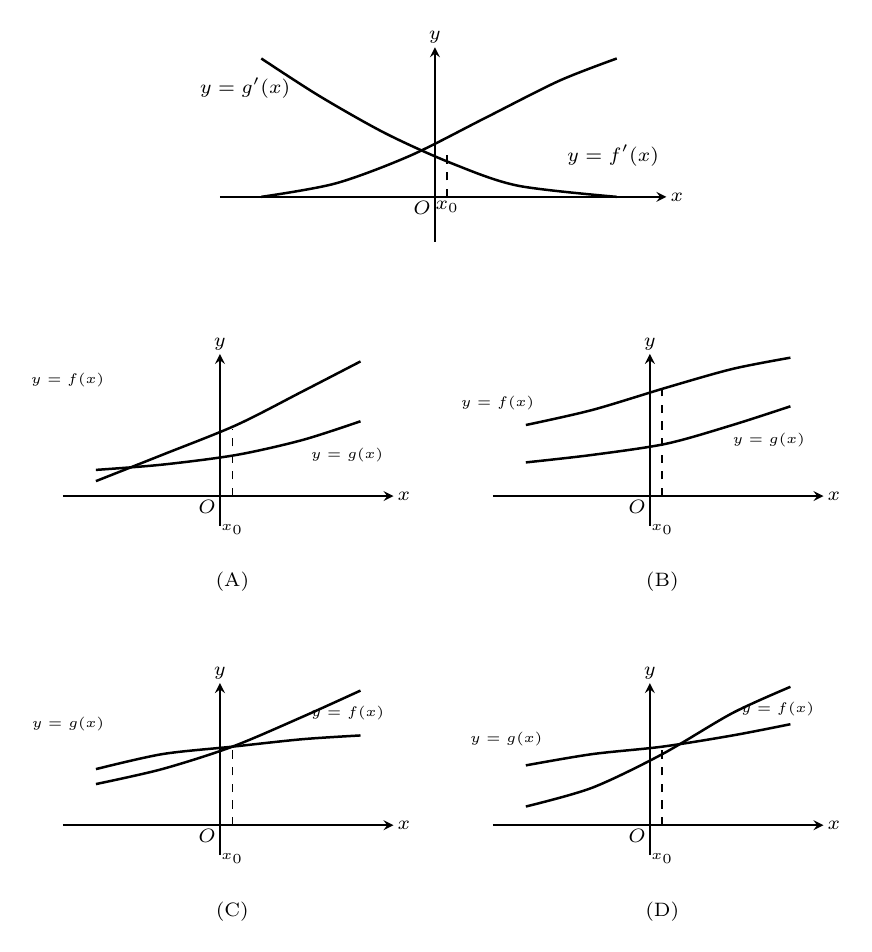
\begin{tikzpicture}[x=1.05cm, y=0.95cm, semithick, font=\scriptsize,
  every node/.style={inner sep=1.2pt}]

  % ---- 题干：导函数图象 ----
  \begin{scope}[shift={(0,0)}]
    \draw[->,>=stealth] (-2.6,0) -- (2.8,0) node[right] {$x$};
    \draw[->,>=stealth] (0,-0.6) -- (0,2.0) node[above] {$y$};
    \node[below left] at (0,0) {$O$};
    \draw[line width=0.9pt, smooth, samples=90]
      plot coordinates {(-2.1,1.85) (-1.4,1.35) (-0.6,0.85) (0.2,0.45) (1.0,0.15) (2.2,0.0)};
    \draw[line width=0.9pt, smooth, samples=90]
      plot coordinates {(-2.1,0.0) (-1.2,0.18) (-0.3,0.55) (0.6,1.05) (1.5,1.55) (2.2,1.85)};
    \draw[dashed] (0.15,0) -- (0.15,0.62);
    \node[below] at (0.15,0) {$x_0$};
    \node[right] at (1.55,0.55) {$y=f'(x)$};
    \node[left] at (-1.70,1.45) {$y=g'(x)$};
  \end{scope}

  % ---- (A) ----
  \begin{scope}[shift={(-2.6,-4.0)}]
    \draw[->,>=stealth] (-1.9,0) -- (2.1,0) node[right] {$x$};
    \draw[->,>=stealth] (0,-0.4) -- (0,1.9) node[above] {$y$};
    \node[below left] at (0,0) {$O$};
    \draw[line width=0.9pt, smooth, samples=90]
      plot coordinates {(-1.5,0.2) (-0.7,0.55) (0.2,0.95) (1.0,1.4) (1.7,1.8)};
    \draw[line width=0.9pt, smooth, samples=90]
      plot coordinates {(-1.5,0.35) (-0.7,0.42) (0.2,0.55) (1.0,0.75) (1.7,1.0)};
    \draw[dashed] (0.15,0) -- (0.15,0.9);
    \node at (0.15,-0.45) {\tiny $x_0$};
    \node[left] at (-1.35,1.55) {\tiny $y=f(x)$};
    \node[right] at (1.05,0.55) {\tiny $y=g(x)$};
    \node at (0.15,-1.15) {(A)};
  \end{scope}

  % ---- (B) ----
  \begin{scope}[shift={(2.6,-4.0)}]
    \draw[->,>=stealth] (-1.9,0) -- (2.1,0) node[right] {$x$};
    \draw[->,>=stealth] (0,-0.4) -- (0,1.9) node[above] {$y$};
    \node[below left] at (0,0) {$O$};
    \draw[line width=0.9pt, smooth, samples=90]
      plot coordinates {(-1.5,0.95) (-0.7,1.15) (0.2,1.45) (1.0,1.7) (1.7,1.85)};
    \draw[line width=0.9pt, smooth, samples=90]
      plot coordinates {(-1.5,0.45) (-0.7,0.55) (0.2,0.7) (1.0,0.95) (1.7,1.2)};
    \draw[dashed] (0.15,0) -- (0.15,1.45);
    \node at (0.15,-0.45) {\tiny $x_0$};
    \node[left] at (-1.35,1.25) {\tiny $y=f(x)$};
    \node[right] at (0.95,0.75) {\tiny $y=g(x)$};
    \node at (0.15,-1.15) {(B)};
  \end{scope}

  % ---- (C) ----
  \begin{scope}[shift={(-2.6,-8.4)}]
    \draw[->,>=stealth] (-1.9,0) -- (2.1,0) node[right] {$x$};
    \draw[->,>=stealth] (0,-0.4) -- (0,1.9) node[above] {$y$};
    \node[below left] at (0,0) {$O$};
    \draw[line width=0.9pt, smooth, samples=90]
      plot coordinates {(-1.5,0.55) (-0.7,0.75) (0.15,1.05) (1.0,1.45) (1.7,1.8)};
    \draw[line width=0.9pt, smooth, samples=90]
      plot coordinates {(-1.5,0.75) (-0.7,0.95) (0.15,1.05) (1.0,1.15) (1.7,1.2)};
    \draw[dashed] (0.15,0) -- (0.15,1.05);
    \node at (0.15,-0.45) {\tiny $x_0$};
    \node[left] at (-1.35,1.35) {\tiny $y=g(x)$};
    \node[right] at (1.05,1.5) {\tiny $y=f(x)$};
    \node at (0.15,-1.15) {(C)};
  \end{scope}

  % ---- (D) ----
  \begin{scope}[shift={(2.6,-8.4)}]
    \draw[->,>=stealth] (-1.9,0) -- (2.1,0) node[right] {$x$};
    \draw[->,>=stealth] (0,-0.4) -- (0,1.9) node[above] {$y$};
    \node[below left] at (0,0) {$O$};
    \draw[line width=0.9pt, smooth, samples=90]
      plot coordinates {(-1.5,0.25) (-0.7,0.5) (0.15,0.95) (1.0,1.5) (1.7,1.85)};
    \draw[line width=0.9pt, smooth, samples=90]
      plot coordinates {(-1.5,0.8) (-0.7,0.95) (0.15,1.05) (1.0,1.2) (1.7,1.35)};
    \draw[dashed] (0.15,0) -- (0.15,1.05);
    \node at (0.15,-0.45) {\tiny $x_0$};
    \node[left] at (-1.25,1.15) {\tiny $y=g(x)$};
    \node[right] at (1.05,1.55) {\tiny $y=f(x)$};
    \node at (0.15,-1.15) {(D)};
  \end{scope}
\end{tikzpicture}
\end{center}
\nopagebreak[4]
\end{question}
\gkpart{二、填空题}

\begin{question}
\gkti{13}若 $(x-2)^5=a_5x^5+a_4x^4+a_3x^3+a_2x^2+a_1x+a_0$，则 $a_1+a_2+a_3+a_4+a_5=$\gkblank{}。（用数字作答）

\end{question}
\begin{question}
\gkti{14}若直线 $3x+4y+m=0$ 与圆 $\begin{cases}x=1+\cos\theta,\\ y=-2+\sin\theta,\end{cases}$（$\theta$ 为参数）没有公共点，则实数 $m$ 的取值范围是\gkblank{}。

\end{question}
\begin{question}
\gkti{15}若三棱锥的三个侧面两两垂直，且侧棱长均为 $\sqrt3$，则其外接球的表面积是\gkblank{}。

\end{question}
\begin{question}
\gkti{16}设 $P$ 是一个数集，且至少含有两个数，若对任意 $a$、$b\in P$，都有 $a+b$、$a-b$、$ab$、$\dfrac ab\in P$（除数 $b\neq0$），则称 $P$ 是一个数域。例如有理数集 $\mathbf Q$ 是数域；数集 $F=\{a+b\sqrt2\mid a,b\in\mathbf Q\}$ 也是数域。有下列命题：① 整数集是数域；② 若有理数集 $\mathbf Q\subseteq M$，则数集 $M$ 必为数域；③ 数域必为无限集；④ 存在无穷多个数域。其中正确的命题的序号是\gkblank{}。（把你认为正确的命题的序号填填上）

\end{question}
\gkpart{三、解答题}

\begin{question}
\gkti{17}已知向量 $\boldsymbol m=(\sin A,\cos A)$，$\boldsymbol n=(\sqrt3,-1)$，$\boldsymbol m\cdot\boldsymbol n=1$，且 $A$ 为锐角。

（1）求角 $A$ 的大小；

（2）求函数 $f(x)=\cos 2x+4\cos A\sin x$（$x\in\mathbf R$）的值域。

\Needspace{0.4\textheight}
\end{question}
\begin{question}
\gkti{18}如图，在四棱锥 $P-ABCD$ 中，侧面 $PAD\perp$ 底面 $ABCD$，侧棱 $PA=PD=\sqrt2$，底面 $ABCD$ 为直角梯形，其中 $BC\parallel AD$，$AB\perp AD$，$AD=2AB=2BC=2$，$O$ 为 $AD$ 中点。

（1）求证：$PO\perp$ 平面 $ABCD$；

（2）求异面直线 $PD$ 与 $CD$ 所成角的大小；

（3）线段 $AD$ 上是否存在点 $Q$，使得它到平面 $PCD$ 的距离为 $\dfrac{\sqrt3}{2}$？若存在，求出 $\dfrac{AQ}{QD}$ 的值；若不存在，请说明理由。
\nopagebreak[4]
\begin{center}% 2008 年福建卷理科第 18 题：四棱锥 P-ABCD，侧面 PAD⊥底面 ABCD，PA=PD=√2，
%   底面为直角梯形，BC∥AD，AB⊥AD，AD=2AB=2BC=2，O 为 AD 中点。
% 来源 PDF：gaokaomath-src/普通高考/2008/2008福建理.pdf
% SHA-256：516e8ac8e113868afa9bc4af4724c3b43f22a1f7fecc830a7f3400b8d973d452
% 原页：2008福建理.pdf 第 1 页（A3 三栏）第 3 栏，书页码 441。
% 重绘依据：与文科卷第 19 题同一幅图（同一几何体）：A 左、D 右、O 在 AD 上、B 左下、C 下中、
%   P 在 O 上方；P—A、P—B、P—C、P—D、A—B、B—C、C—D 实线，A—D（含 O）与 P—O 虚线。
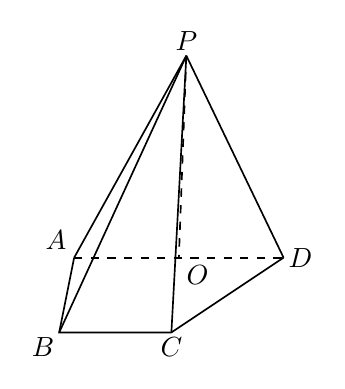
\begin{tikzpicture}[scale=0.95, semithick, every node/.style={inner sep=1.5pt}]
  \coordinate (P) at (1.70,4.00);
  \coordinate (A) at (0.20,1.30);
  \coordinate (D) at (3.00,1.30);
  \coordinate (O) at (1.60,1.30);
  \coordinate (B) at (0.00,0.30);
  \coordinate (C) at (1.50,0.30);

  \draw (P) -- (A);
  \draw (P) -- (B);
  \draw (P) -- (C);
  \draw (P) -- (D);
  \draw (A) -- (B) -- (C) -- (D);
  \draw[dashed] (A) -- (D);
  \draw[dashed] (P) -- (O);

  \node[above] at (P) {$P$};
  \node[above left=1pt] at (A) {$A$};
  \node[right] at (D) {$D$};
  \node[below right=1pt] at (O) {$O$};
  \node[below left] at (B) {$B$};
  \node[below] at (C) {$C$};
\end{tikzpicture}
\end{center}
\nopagebreak[4]
\end{question}
\begin{question}
\gkti{19}已知函数 $f(x)=\dfrac13x^3+x^2-2$。

（1）设 $\{a_n\}$ 是正数组成的数列，前 $n$ 项和为 $S_n$，其中 $a_1=3$。若点 $(a_n,a_{n+1}^2-2a_{n+1})$（$n\in\mathbf N^*$）在函数 $y=f'(x)$ 的图象上，求证：点 $(n,S_n)$ 也在 $y=f'(x)$ 的图象上；

（2）求函数 $f(x)$ 在区间 $(a-1,a)$ 内的极值。

\end{question}
\begin{question}
\gkti{20}某项考试按科目 $A$、科目 $B$ 依次进行，只有当科目 $A$ 成绩合格时，才可继续参加科目 $B$ 的考试。已知每个科目只允许有一次补考机会，两个科目成绩均合格方可获得证书。现某人参加这项考试，科目 $A$ 每次考试成绩合格的概率均为 $\dfrac23$，科目 $B$ 每次考试成绩合格的概率均为 $\dfrac12$。假设各次考试成绩合格与否均互不影响。

（1）求他不需要补考就可获得证书的概率；

（2）在这项考试过程中，假设他不放弃所有的考试机会，记他参加考试的次数为 $\xi$，求 $\xi$ 的数学期望 $E\xi$。

\Needspace{0.4\textheight}
\end{question}
\begin{question}
\gkti{21}如图，椭圆 $\dfrac{x^2}{a^2}+\dfrac{y^2}{b^2}=1$（$a>b>0$）的一个焦点是 $F(1,0)$，$O$ 为坐标原点。

（1）已知椭圆短轴的两个三等分点与一个焦点构成正三角形，求椭圆的方程；

（2）设过点 $F$ 的直线 $l$ 交椭圆于 $A$、$B$ 两点。若直线 $l$ 绕点 $F$ 任意转动，恒有 $|OA|^2+|OB|^2<|AB|^2$，求 $a$ 的取值范围。
\nopagebreak[4]
\begin{center}% 2008 年福建卷理科第 21 题：椭圆 x²/a²+y²/b²=1（a>b>0），焦点 F(1,0)，O 为原点；
%   过 F 的直线 l 交椭圆于 A、B。
% 来源 PDF：gaokaomath-src/普通高考/2008/2008福建理.pdf
% SHA-256：516e8ac8e113868afa9bc4af4724c3b43f22a1f7fecc830a7f3400b8d973d452
% 原页：2008福建理.pdf 第 2 页（A3 三栏）第 2 栏，书页码 442。
% 重绘依据：按原页画椭圆与 x/y 轴，F 在 x 轴正半轴上；过 F 的直线 l 与椭圆交于
%   第一象限的 A 与第三象限的 B。取图示椭圆 x 半径 2.6、y 半径 1.75，A、B 取在椭圆上
%   且与 F 共线（A≈(1.99,1.13)、B≈(−0.51,−1.72)），l 在两端各延长一小段。
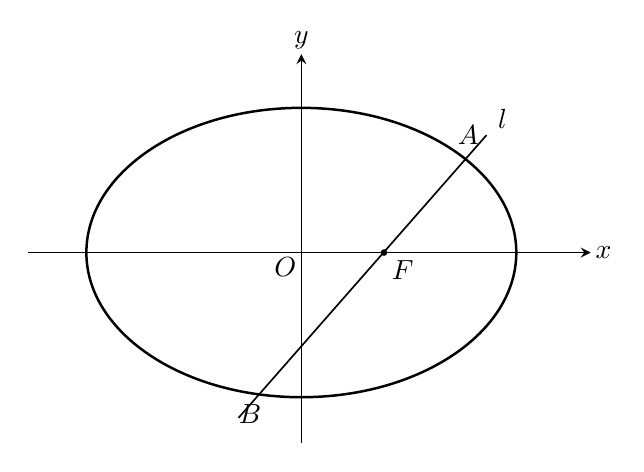
\begin{tikzpicture}[x=1.05cm, y=1.05cm, semithick, every node/.style={inner sep=1.5pt}]
  \draw[->,>=stealth] (-3.3,0) -- (3.5,0) node[right] {$x$};
  \draw[->,>=stealth] (0,-2.3) -- (0,2.4) node[above] {$y$};
  \node[below left] at (0,0) {$O$};

  \draw[line width=0.9pt] (0,0) ellipse [x radius=2.6, y radius=1.75];

  \coordinate (F) at (1,0);
  \coordinate (A) at (1.99,1.13);
  \coordinate (B) at (-0.51,-1.72);

  \draw (-0.76,-2.00) -- (2.24,1.42);
  \node[right] at (2.32,1.62) {$l$};

  \fill (F) circle (1.2pt);
  \node[below right=1pt] at (F) {$F$};
  \node at (2.02,1.42) {$A$};
  \node at (-0.62,-1.95) {$B$};
\end{tikzpicture}
\end{center}
\nopagebreak[4]
\end{question}
\begin{question}
\gkti{22}已知函数 $f(x)=\ln(1+x)-x$。

（1）求 $f(x)$ 的单调区间；

（2）记 $f(x)$ 在区间 $[0,\pi]$（$n\in\mathbf N^*$）上的最小值为 $b_n$，令 $a_n=\ln(1+n)-b_n$。

① 如果对一切 $n$，不等式 $\sqrt{a_n}<\sqrt{a_{n+2}}-\dfrac{c}{\sqrt{a_{n+2}}}$ 恒成立，求实数 $c$ 的取值范围；

② 求证：$\dfrac{a_1}{a_2}+\dfrac{a_1a_3}{a_2a_4}+\cdots+\dfrac{a_1a_3\cdots a_{2n-1}}{a_2a_4\cdots a_{2n}}<\sqrt{2a_n+1}-1$。

\end{question}